\documentclass[11pt,a4paper,onecolumn]{article}
\usepackage[left=2cm,text={17cm,24cm},top=3cm]{geometry}

\usepackage[czech]{babel}
\usepackage[utf8]{inputenc}
\usepackage{times}
\usepackage{amsthm}
\usepackage{amsmath}
\usepackage{amssymb}
\usepackage{array}
\usepackage{multirow}
\usepackage{dcolumn}
\usepackage[czech,ruled,linesnumbered,longend,noline]{algorithm2e}
\usepackage{graphics}
\usepackage{float}
\usepackage{picture}



\begin{document}
\begin{titlepage}
  \begin{center}

    \textsc{\Huge Vysoké učení technické v~Brně\\\huge Fakulta informačních technologií}\\
    \vspace{\stretch{0.382}}\LARGE Typografie a publikování -- 3. projekt\\\Huge
    Tabulky a obrázky\vspace{\stretch{0.618}}\\
  \end{center}
  {\Large 27. března 2015 \hfill Vojtěch Večeřa}
\end{titlepage}

\section{Úvodní stránka}
\label{uvod}
\noindent Název práce umístěte do zlatého řezu a nezapomeňte uvést dnešní datum a vaše jméno a příjmení.
\section{Tabulky}
\label{tabulky}
\noindent Pro sázení tabule můžeme použít buď prostředí \texttt{tabbing} nebo prostředí \texttt{tabular}.
\subsection{Prostředí \texttt{tabbing}}
\noindent Při použití\texttt{ tabbing }vypadá tabulka následovně:
\begin{tabbing}
\pushtabs \qquad\qquad\qquad\qquad \= \qquad\qquad \= \qquad\qquad \kill
\textbf{Ovoce} \> \textbf{Cena} \> \textbf{Množství} \\
Jablka \> 25,90 \> 3 kg \\
Hrušky \> 27,40 \> 2,5 kg \\
Vodní melouny \> 35,-- \> 1 kus \\
\poptabs
\end{tabbing}
\noindent Toto prostředí se dá také pro sázení algoritmů, ovšem vhodnější je použít prostředí \texttt{algorithm} nebo \texttt{algorithm2e} (viz sekce \ref{algo}).
\subsection{Prostředí \texttt{tabular}}
\noindent Další možností jak vytvořit tabulku, je použít prostředí \texttt{tabular}. Tabulky pak budou vypadat takto\footnote{Kdyby byl problém s \texttt{cline}, zkuste se podívat třeba sem: http://www.abclinux.cz/tex/poradna/show/325037.}:

\begin{table}[ht]

\catcode`\-=12
\begin{center}
\begin{tabular}[p]{| c | c | c |}

\hline 
& \multicolumn{2}{c|}{\bfseries Cena} \\\cline{2-3}
\textbf{Měna} &  \textbf{nákup} & \textbf{prodej} \\\hline
EUR  & 27,34 & 27,42 \\
GBP  & 33,09 & 33,41 \\
USD  & 19,87 & 19,05 \\\hline
\end{tabular}
\caption{Tabulka kurzů k dnešnímu dni}
\label{tab1}
\end{center}
\end{table}

\begin{table}[ht]

\begin{center}
\catcode`\-=12
\begin{tabular}[p]{|>{\bfseries}c|c|}\hline

$A$ & $\neg A$ \\\hline
P & N \\\hline
O & O \\\hline
X & X \\\hline
N & P \\\hline
\end{tabular}
\begin{tabular}[p]{|c|>{\bfseries}c|c|c|c|c|}\hline
\multicolumn{2}{|c|}{\multirow{2}{*}{$A \wedge B$}} & \multicolumn{4}{c|}{$B$} \\\cline{3-6}
\multicolumn{2}{|c|}{} & \textbf{P} & \textbf{O} & \textbf{X} & \textbf{N}  \\\hline
\multirow{4}{*}{A} 
  & P & P & O & X & N\\\cline{2-6}
  & O & O & O & N & N\\\cline{2-6}
  & X & X & N & X & N\\\cline{2-6}
  & N & N & N & N & N\\\hline
\end{tabular}
\begin{tabular}[p]{|c|>{\bfseries}c|c|c|c|c|}\hline
\multicolumn{2}{|c|}{\multirow{2}{*}{$A \vee B$}} & \multicolumn{4}{c|}{$B$} \\\cline{3-6}
\multicolumn{2}{|c|}{} & \textbf{P} & \textbf{O} & \textbf{X} & \textbf{N}  \\\hline
\multirow{4}{*}{A} 
  & P & P & P & P & P\\\cline{2-6}
  & O & P & O & P & O\\\cline{2-6}
  & X & P & P & X & X\\\cline{2-6}
  & N & P & O & X & N\\\hline
\end{tabular}
\begin{tabular}[p]{|c|>{\bfseries}c|c|c|c|c|}\hline
\multicolumn{2}{|c|}{\multirow{2}{*}{$A \rightarrow B$}} & \multicolumn{4}{c|}{$B$} \\\cline{3-6}
\multicolumn{2}{|c|}{} & \textbf{P} & \textbf{O} & \textbf{X} & \textbf{N}  \\\hline
\multirow{4}{*}{A} 
  & P & P & O & X & N\\\cline{2-6}
  & O & P & O & P & O\\\cline{2-6}
  & N & P & P & X & X\\\cline{2-6}
  & X & P & P & P & P\\\hline
\end{tabular}
\caption{Protože Kleeneho trojhodnotová logika už je "zastaralá", uvádíme si zde příklad čtyřhodnotové logiky}
\label{tab2}
\end{center}
\end{table}

\section{Algoritmy}
\label{algo}
\noindent Pokud budeme chtít vysázet algoritmus, můžeme použít prostředí \texttt{algorithm}\footnote{\raggedright Pro nápovědu, jak zacházet s prostředím \texttt{algorithm}, můžeme zkusit tuhle stránku: http://ftp.cstug.cz/pub/tex/CTAN/macros/latex/contrib/algorithms/algorithms.pdf.}
nebo \texttt{algorithm2e}\footnote{\raggedright Pro \texttt{algorithm2e} zase tuhle: http://ftp.cstug.cz/pub/tex/CTAN/macros/latex/contrib/algorithm2e/doc/algorithm2e.pdf.}
Příklad použití prostředí \texttt{algorithm2e} viz Algoritmus \ref{alg1}.

\vspace{1.5em}
\IncMargin{1em}
\begin{algorithm}[H]
\label{alg1}
\DontPrintSemicolon
\SetNlSty{}{}{:}
\SetAlgoNlRelativeSize{0}
\KwIn{$(X_{t-1}, v_t, z_t)$}
\KwOut{$X_t$}
$\overline{X} = X = 0$ \;
\For{$k = 1$ \KwTo $M$}{
$x_t^{[k]} = sample\_motion\_model (u_t, x_{t-1}^{[k]}) $\;
$w_t^{[k]} = measurement\_model (z_t, x_t^{[k]}, m_{t-1}) $\;
$m_t^{[k]} = updated\_occupancy\_grid (z_t, x_t^{[k]},m_{t-1}^{[k]}) $\;
$\overline{X_t} = \overline{X_t} + \langle x_x^{[m]}, w_t{[m]} \rangle $\;
}
\For{k = 1 \KwTo $M$}{
draw $ i $ with probability $ \approx w_i^{[i]} $\;
add $ \langle x_{x}^{[k]}, m_{i}^{[k]} \rangle$ \KwTo $ X_i $ \;
}
\KwRet $X_t$\;
\caption{\textsc{FastSLAM}}
\end{algorithm}

\DecMargin{1em}
\vspace{1.5em}


\section{Obrázky}
\label{obr}
\noindent Do našich článků můžeme samozřejmě vkládat obrázky. Pokud je obrázkem fotografie, můžeme klidně použít bitmapový soubor. Pokud by to ale mělo být nějaké schéma nebo něco podobného, je dobrým zvykem takovýto obrázek vytvořit vektorově.

\begin{figure}[H]
\begin{center}
\scalebox{0.4}{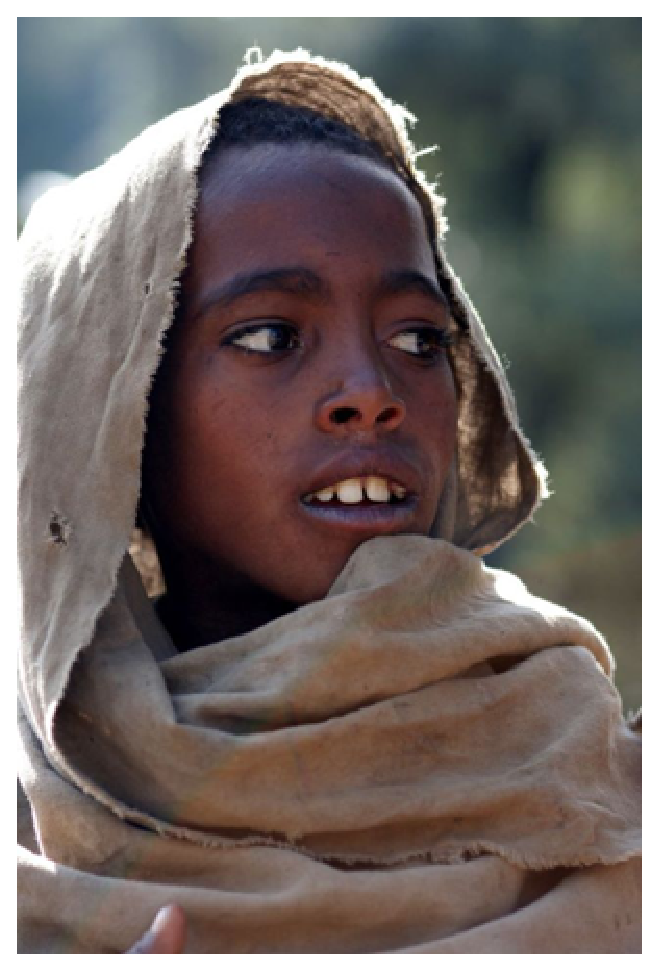
\includegraphics{etiopan.eps}\reflectbox{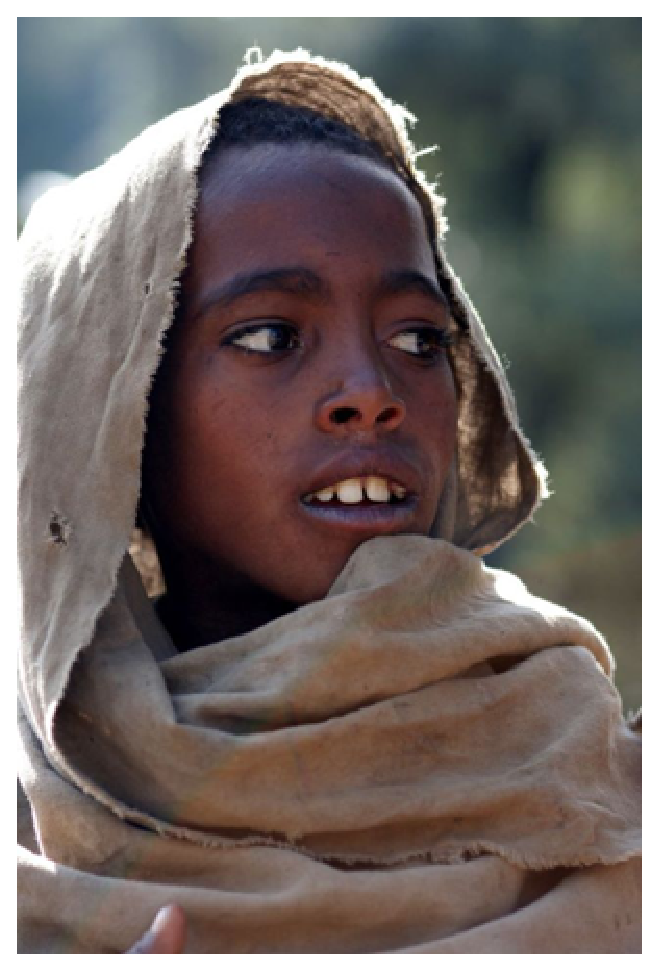
\includegraphics{etiopan.eps}}}
\caption{Malý etiopánek a jeho bratříček}
\label{obr1}
\end{center}
\end{figure}

\noindent Rozdíl mezi vektorovým\dots

\begin{figure}[H]
\begin{center}
\scalebox{0.33}{

\includegraphics{oniisan.eps}}
\end{center}
\caption{Vektorový obrázek}
\label{obr2}
\end{figure}

\noindent\dots a bitmapovým obrázkem

\begin{figure}[H]
\begin{center}
\scalebox{0.5}{

\includegraphics{oniisan2.eps}}
\end{center}
\caption{Bitmapový obrázek}
\label{obr3}
\end{figure}

\noindent se projeví například při zvětšení.


Odkazy (nejen ty) na obrázky \ref{obr1}, \ref{obr2}, a \ref{obr3}, na tabulky \ref{tab1} a \ref{tab2} a také na algoritmus \ref{alg1} jsou udělány pomocí křížových odkazů. Pak je ovšem potřeba zdrojový soubor přeložit dvakrát.
\indent Vektorové obrázky lze vytvořit i přímo v \LaTeX u, například v prostředí \texttt{picture}. Všechny rozmery jsou uváděny v mm.

\begin{figure}
\begin{center}
\setlength{\unitlength}{1.35mm}
\begin{picture}(115,158.5)

\linethickness{1.35mm}
\thinlines
\multiput(15,2)(0,9.9){16}{\line(0,1){7.5}}
\multiput(0,144)(9.9,0){11}{\line(1,0){7.5}}

\put(98,151.25){\makebox(0,0){\shortstack{Výška\\mezery = 14.5}}}
\put(88,151.25){\vector(0,1){7.25}\vector(0,-1){7.25}}
\put(97,139){\makebox(0,0){\shortstack{Výška\\mezery = 10}}}
\put(88,139){\vector(0,1){5}\vector(0,-1){5}}
\put(97,129){\makebox(0,0){\shortstack{Výška\\hlavičky = 10}}}
\put(88,129){\vector(0,1){5}\vector(0,-1){5}}
\put(97,117){\makebox(0,0){\shortstack{Výška\\mezery = 14}}}
\put(88,117){\vector(0,1){7}\vector(0,-1){7}}
\put(94,72.5){\makebox(0,0){\shortstack{Výška\\těla = 75}}}
\put(88,72.5){\vector(0,1){37.5}\vector(0,-1){37.5}}
\put(97,27.5){\makebox(0,0){\shortstack{Výška\\mezery = 15}}}
\put(88,27.5){\vector(0,1){7.5}\vector(0,-1){7.5}}
\put(95,15){\makebox(0,0){\shortstack{Výška\\paty = 10}}}
\put(88,15){\vector(0,1){5}\vector(0,-1){5}}
\put(100,55){\makebox(0,0){\shortstack{Výška\\stránky = 158.5}}}
\put(100,59){\vector(1,1){12}}
\put(112,79.25){\vector(0,1){79.25}\vector(0,-1){79.25}}

\put(57.5,140){\makebox(0,0){Šířka boxu = 55}}
\put(57.5,137){\vector(1,0){27.5}}
\put(57.5,137){\vector(-1,0){27.5}}
\put(98,105){\makebox(0,0){Mezera = 9}}
\put(94,103){\vector(-1,-4){2.5}}
\put(89.5,93){\vector(1,0){4.5}\vector(-1,0){9}}
\put(7.5,95){\makebox(0,0){Mezera = 15}}
\put(0,93){\vector(1,0){15}\vector(-1,0){15}}
\put(101.5,97){\makebox(0,0){\shortstack{Šířka\\boxu = 15}}}
\put(94,93){\vector(1,0){15}\vector(-1,0){15}}
\put(57.5,5){\makebox(0,0){Šířka stránky = 115}}
\put(0,3){\vector(1,0){115}\vector(-1,0){115}}

\thicklines

\put(0,0){\framebox(115,158.5){}}
\put(30,124){\framebox(55,10){\textbf{Hlavička}}}
\put(30,35){\framebox(55,75){\textbf{Textové tělo}}}
\put(94,79){\framebox(15,10){\shortstack{\bfseries Okrajová\\*\bfseries poznámka}}}
\put(30,10){\framebox(55,10){\textbf{Pata}}}




\end{picture}
\caption{Vektorový obrázek v prostředí \texttt{picture}.}
\end{center}
\end{figure}


\end{document}
